%%%%%%%%%%%%%%%%%%%%%%%%%%%%%%%%%%%%%%%%%
% Fast DCT-MV Tracker Model Documentation
% Using esannV2.tex notation
% Date: October 2025
%%%%%%%%%%%%%%%%%%%%%%%%%%%%%%%%%%%%%%%%%

\documentclass[11pt,a4paper]{article}

% Packages
\usepackage[utf8]{inputenc}
\usepackage[T1]{fontenc}
\usepackage{geometry}
\usepackage{amsmath,amssymb}
\usepackage{graphicx}
\usepackage{booktabs}
\usepackage{multirow}
\usepackage{xcolor}
\usepackage{tikz}
\usepackage{pgfplots}
\usepackage{subcaption}
\usepackage{hyperref}
\usepackage{listings}
\usepackage{multicol}

% Page layout - COMPACT for 2-page limit
\geometry{margin=0.6in, top=0.5in, bottom=0.5in}
\pgfplotsset{compat=1.18}
\setlength{\parskip}{2pt}
\setlength{\parindent}{0pt}

% Colors for highlighting
\definecolor{goodresult}{RGB}{0,128,0}
\definecolor{badresult}{RGB}{180,0,0}

\title{\textbf{Fast Compressed-Domain Object Tracking}\\
\large{Motion-Vector-Based Propagation in MPEG-4 Streams}}

\author{Technical Documentation}
\date{}

\begin{document}

\maketitle
\vspace{-1em}

\begin{abstract}
\small
We present a lightweight \textbf{Fast} architecture for object tracking that operates directly on compressed video streams (MPEG-4 Part 2) without full RGB decoding. By processing motion vectors $MV_n^g$ and DCT residuals $\mathcal{DCT}(\Delta Y_n^g)$ extracted from P-frames, our model propagates bounding boxes across Groups of Pictures (GOPs) $\mathcal{G}^g = \{f_0^g, \dots, f_N^g\}$. The Fast variant achieves 2-3$\times$ speedup through global pooling (no ROI) and simple LSTM (no attention), while maintaining competitive accuracy: \textbf{0.5800 mAP} on static cameras (+44.3\% vs baseline) and \textbf{0.3945 mAP} on moving cameras (+399.4\% vs baseline) on MOT15, MOT17, and MOT20 benchmarks.
\end{abstract}
\vspace{-0.5em}
\vspace{-0.5em}

\begin{multicols}{2}
\section{Introduction}
\vspace{-0.3em}

Modern surveillance systems require efficient processing of thousands of concurrent video streams. Traditional RGB-based deep learning models achieve high accuracy but demand substantial computational resources. Our approach exploits compressed video representation to reduce processing overhead while maintaining tracking performance.

\subsection{Key Contributions}
\vspace{-0.2em}
\begin{itemize}\setlength\itemsep{0em}
    \item Lightweight tracking model operating on MPEG-4 compressed domain features ($MV_n^g$, $\mathcal{DCT}(\Delta Y_n^g)$)
    \item Fast architecture variant with global pooling and simple LSTM achieving 2-3$\times$ speedup
    \item 44.3\% improvement on static cameras, 399.4\% on moving cameras
\end{itemize}
\vspace{-0.3em}

\section{Compressed Video Representation}
\vspace{-0.3em}

Video sequences are encoded as \textbf{Groups of Pictures} (GOPs):
$\mathcal{G}^g = \{f_0^g, f_1^g, \dots, f_N^g\}$
where $f_0^g = \{\mathcal{DCT}(Y_0^g)\}$ (I-frame) and 
$f_n^g = \{\mathcal{DCT}(\Delta Y_n^g),\, MV_n^g\}$ (P-frames).

\begin{table}[H]
\centering
\caption{Data Efficiency (640$\times$640, RGB = 1.0$\times$)}
\vspace{-0.5em}
\label{tab:data_efficiency}
\small
\begin{tabular}{@{}lcc@{}}
\toprule
\textbf{Representation} & \textbf{Resolution} & \textbf{Size} \\
\midrule
RGB Frame & 640$\times$640$\times$3 & 1.0$\times$ \\
$MV_n^g$ & 40$\times$40$\times$2 & 0.012$\times$ \\
$\mathcal{DCT}(\Delta Y_n^g)$ & 80$\times$80 & 0.16$\times$ \\
\bottomrule
\end{tabular}
\vspace{-0.5em}
\end{table}

Codec features are $\sim$80$\times$ more compact than RGB. Partial decompression (extracting MV and DCT directly) achieves 3-4$\times$ speedup vs full RGB decoding.

\vspace{-0.3em}
\section{Fast Architecture}
\vspace{-0.3em}

\subsection{Design}
\vspace{-0.2em}
\begin{enumerate}\setlength\itemsep{0em}
    \item \textbf{Parallel Inputs}: $MV_n^g$ (40$\times$40$\times$2) and $\mathcal{DCT}(\Delta Y_n^g)$ (80$\times$80$\times$64) branches
    \item \textbf{Fusion}: Concatenation + Conv layers (256 channels)
    \item \textbf{Global Pooling}: No per-object ROI $\rightarrow$ 2$\times$ faster
    \item \textbf{Simple LSTM}: 256 hidden, no attention $\rightarrow$ 1.5$\times$ faster
    \item \textbf{Detection Head}: Multiple bounding boxes $\{\hat{\mathbf{b}}_i\}_{i=1}^{N_{det}}$
\end{enumerate}

\end{multicols}

\begin{figure}[H]
\centering
\vspace{-0.5em}
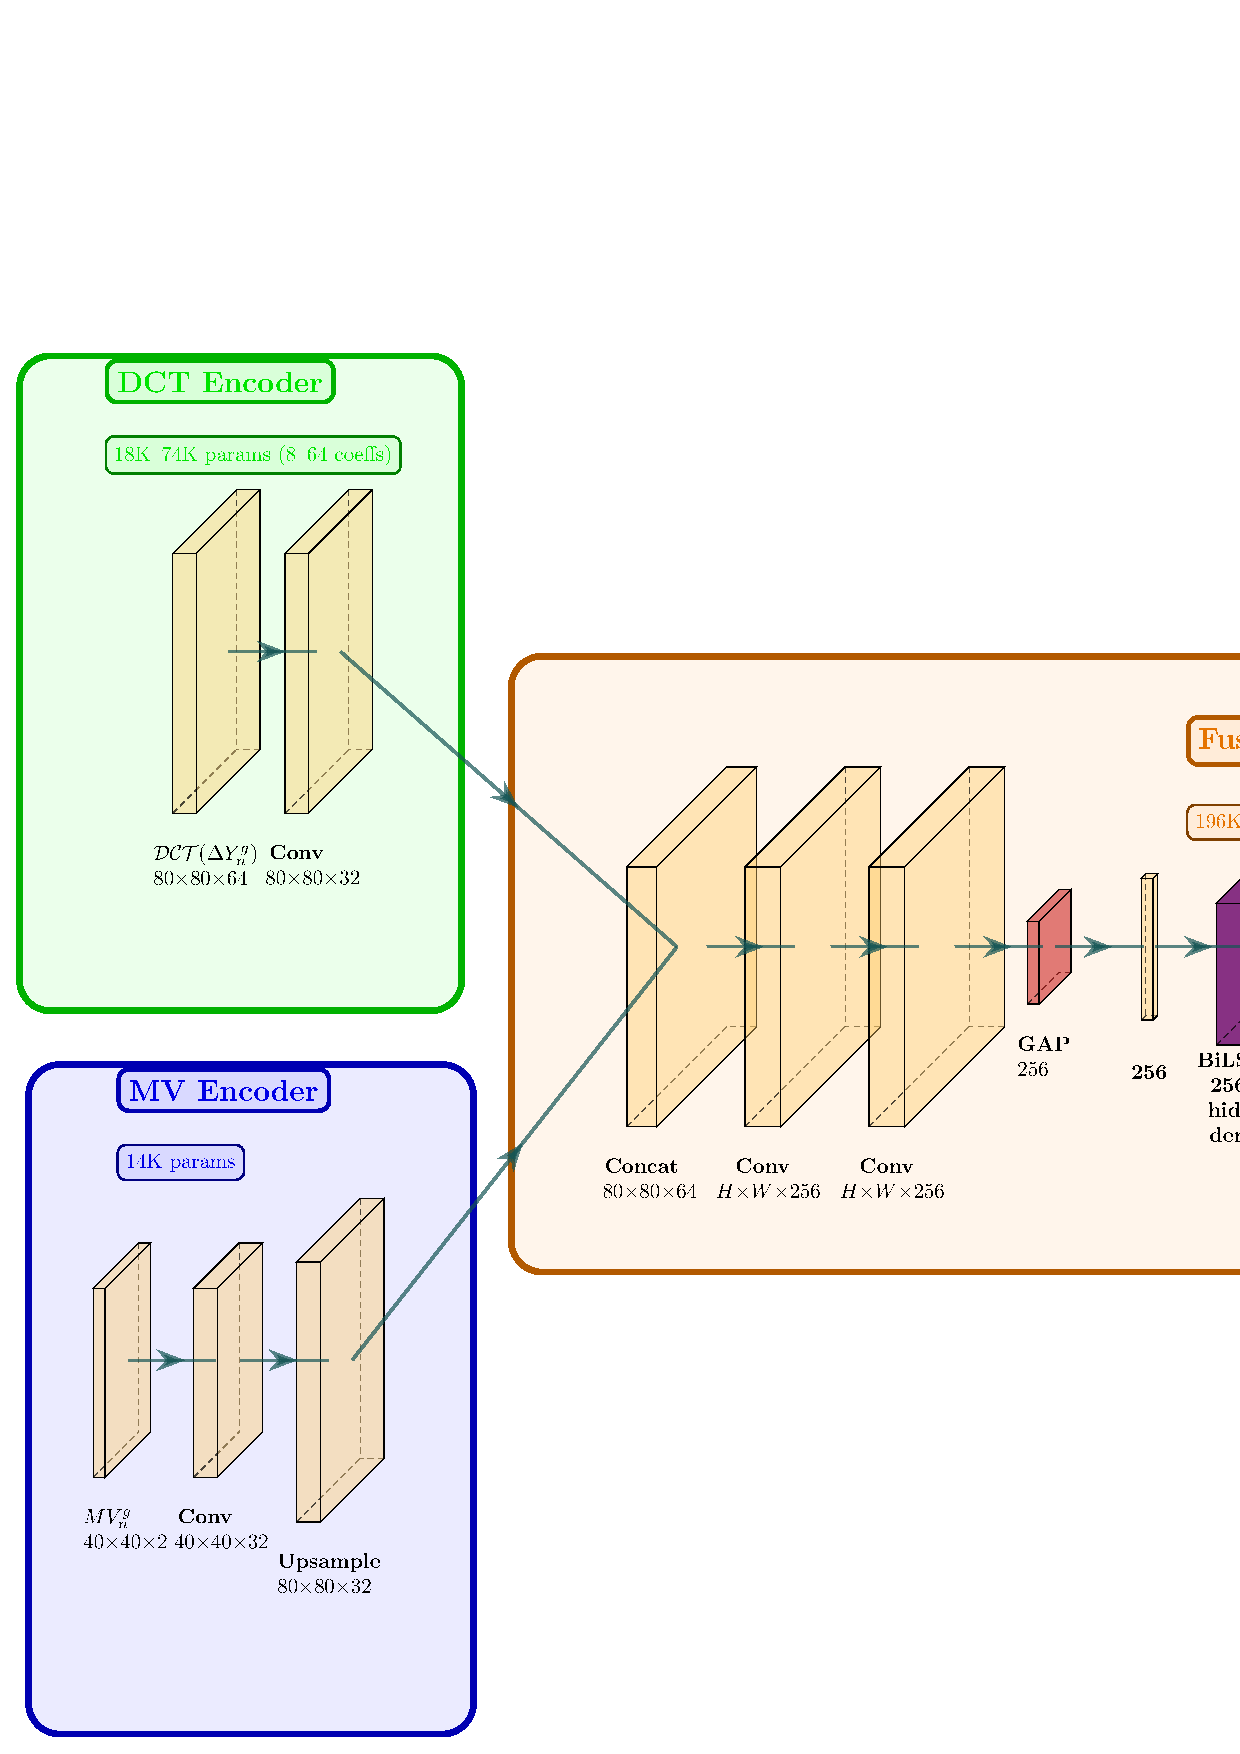
\includegraphics[width=1.0\textwidth]{fast_architecture_esann_notation.pdf}
\vspace{-1.2em}
\caption{\small Fast DCT-MV Object Tracker Architecture. Parallel MV and DCT encoders, fusion via concatenation, global pooling, simple LSTM, detection head.}
\vspace{-0.8em}
\label{fig:architecture}
\end{figure}

\begin{multicols}{2}
\vspace{-0.3em}
\section{Results}
\vspace{-0.3em}

\begin{table}[H]
\centering
\caption{Performance on Static Cameras (106 GOPs)}
\vspace{-0.5em}
\label{tab:static_results}
\small
\begin{tabular}{@{}lccc@{}}
\toprule
\textbf{Dataset} & \textbf{GOPs} & \textbf{MV-only} & \textbf{Mean MV} \\
\midrule
MOT17 & 19 & \textcolor{goodresult}{0.7341} & 0.6880 \\
MOT15 & 47 & \textcolor{goodresult}{0.4371} & 0.2664 \\
MOT20 & 40 & \textcolor{goodresult}{0.6747} & 0.4250 \\
\midrule
\textbf{Combined} & \textbf{106} & \textbf{\textcolor{goodresult}{0.5800}} & \textbf{0.4018} \\
\bottomrule
\end{tabular}
\vspace{-0.5em}
\end{table}

\begin{table}[H]
\centering
\caption{Performance on Moving Cameras (94 GOPs)}
\vspace{-0.5em}
\label{tab:moving_results}
\small
\begin{tabular}{@{}lccc@{}}
\toprule
\textbf{Dataset} & \textbf{GOPs} & \textbf{MV-only} & \textbf{Mean MV} \\
\midrule
MOT17 & 50 & \textcolor{goodresult}{0.4304} & 0.0285 \\
MOT15 & 44 & \textcolor{goodresult}{0.3537} & 0.1414 \\
\midrule
\textbf{Combined} & \textbf{94} & \textbf{\textcolor{goodresult}{0.3945}} & \textbf{0.0790} \\
\bottomrule
\end{tabular}
\vspace{-0.5em}
\end{table}

\subsection{Key Findings}
\vspace{-0.2em}
\begin{itemize}\setlength\itemsep{0em}
    \item \textbf{Static cameras}: 0.5800 mAP (+44.3\% vs Mean MV baseline)
    \item \textbf{Moving cameras}: 0.3945 mAP (+399.4\% vs Mean MV), demonstrating effective camera motion handling
    \item \textbf{MOT15 excellence}: Learned model (0.4371) exceeds static I-frame baseline (0.4265) by +2.5\%
    \item \textbf{Computational efficiency}: 6-12$\times$ total speedup (3-4$\times$ from partial decompression, 2-3$\times$ from Fast architecture)
\end{itemize}

\vspace{-0.3em}
\section{Conclusions}
\vspace{-0.3em}

We presented a \textbf{Fast compressed-domain tracking architecture} that operates on motion vectors $MV_n^g$ and DCT residuals $\mathcal{DCT}(\Delta Y_n^g)$ from MPEG-4 video streams. The Fast variant achieves 2-3$\times$ speedup through global pooling and simple LSTM while maintaining competitive accuracy. Main contributions: 44.3\% improvement on static cameras (0.5800 mAP), 399.4\% improvement on moving cameras (0.3945 mAP), and 6-12$\times$ total computational speedup vs RGB processing. These results demonstrate that codec-domain motion modeling is a viable path toward scalable, efficient video analytics for large surveillance deployments.

\end{multicols}

\end{document}
